% Preámbulo
\documentclass[stu, 12pt, letterpaper, donotrepeattitle, floatsintext, natbib]{apa7}
\usepackage[utf8]{inputenc}
\usepackage{comment}
\usepackage{marvosym}
\usepackage{graphicx}
\usepackage{float}
\usepackage{amsmath}
\usepackage[normalem]{ulem}
\usepackage[spanish]{babel} 
\usepackage{indentfirst} %para le formato que quiere la profe QUITAR SI QUIERES OG APA7
\usepackage{ragged2e} %para le formato que quiere la profe QUITAR SI QUIERES OG APA7
\usepackage{indentfirst} %para le formato que quiere la profe QUITAR SI QUIERES OG APA7
\usepackage{multirow,booktabs,setspace,caption} %formato de figuras APA
\DeclareCaptionLabelSeparator*{spaced}{\\[2ex]}
\DeclareCaptionLabelSeparator*{spaced}{\\[2ex]}
\captionsetup[figure]{textfont=it,format=plain,justification=justified,
  singlelinecheck=false,labelsep=spaced,skip=0pt}

\selectlanguage{spanish}
\useunder{\uline}{\ul}{}
\newcommand{\myparagraph}[1]{\paragraph{#1}\mbox{}\\}

% Portada
%\thispagestyle{empty}
\title{\Large Tarea 2 Unidad 3: Objetos trdimensionales}
\author{Abraham Jhared Flores Azcona} % (autores separados, consultar al docente)
% Manera oficial de colocar los autores:
%\author{Autor(a) I, Autor(a) II, Autor(a) III, Autor(a) X}
\affiliation{Instituto Tecnológico de Tijuana}
\course{SCC-1010SC5C: Graficación}
\professor{Dra. Martha Elena Pulido}
\duedate{13 de septiembre de 2021}

\begin{document}
    % Índices
    \pagenumbering{arabic}
    \maketitle

    % Contenido
    \renewcommand\contentsname{Contenido}
    \tableofcontents
    \renewcommand{\listfigurename}{Figuras}
    \listoffigures

    % Cuerpo 
    %NOTA: PARA CITAR ESTILO "Merts (2003)" usar \cite{<nombre_cita_bib>}
    %    
    \newpage
    \section*{Introducción}
    Es \begin{justifying}
        indudable que los medios de entretenimiento que han ganado mayor popularidad han sido aquellos de los gráficos tridimensionales.
        Por ello es de suma importancia conocer como se representan, sus técnicas de visualización así como los elementos necesarios para 
        su análisis son relevantes para nuestros estudios, los cuales se resumen a continuación.\par
    \end{justifying}
    \vspace{\baselineskip}
    \section{Representación de objetos en tres dimensiones}
    A \begin{justifying}
        grandes rasgos, un objeto tridimensional consta de 3 ejes en los cuales se va a
        poder representar su posición en el espacio. Aparte de esto, los conjuntos tridimensionales de datos
        en el ecosistema computarizado se encuentran en diferentes formas que varian a la vez en la estructura
        y propiedades \citep{poux-2021}.\par %citar al frances
    \end{justifying}
    \vspace{\baselineskip}
    \begin{figure}[H]
        \caption{\emph{Representaciones de datos tridimensionales como objetos 3D}}
        \centering
        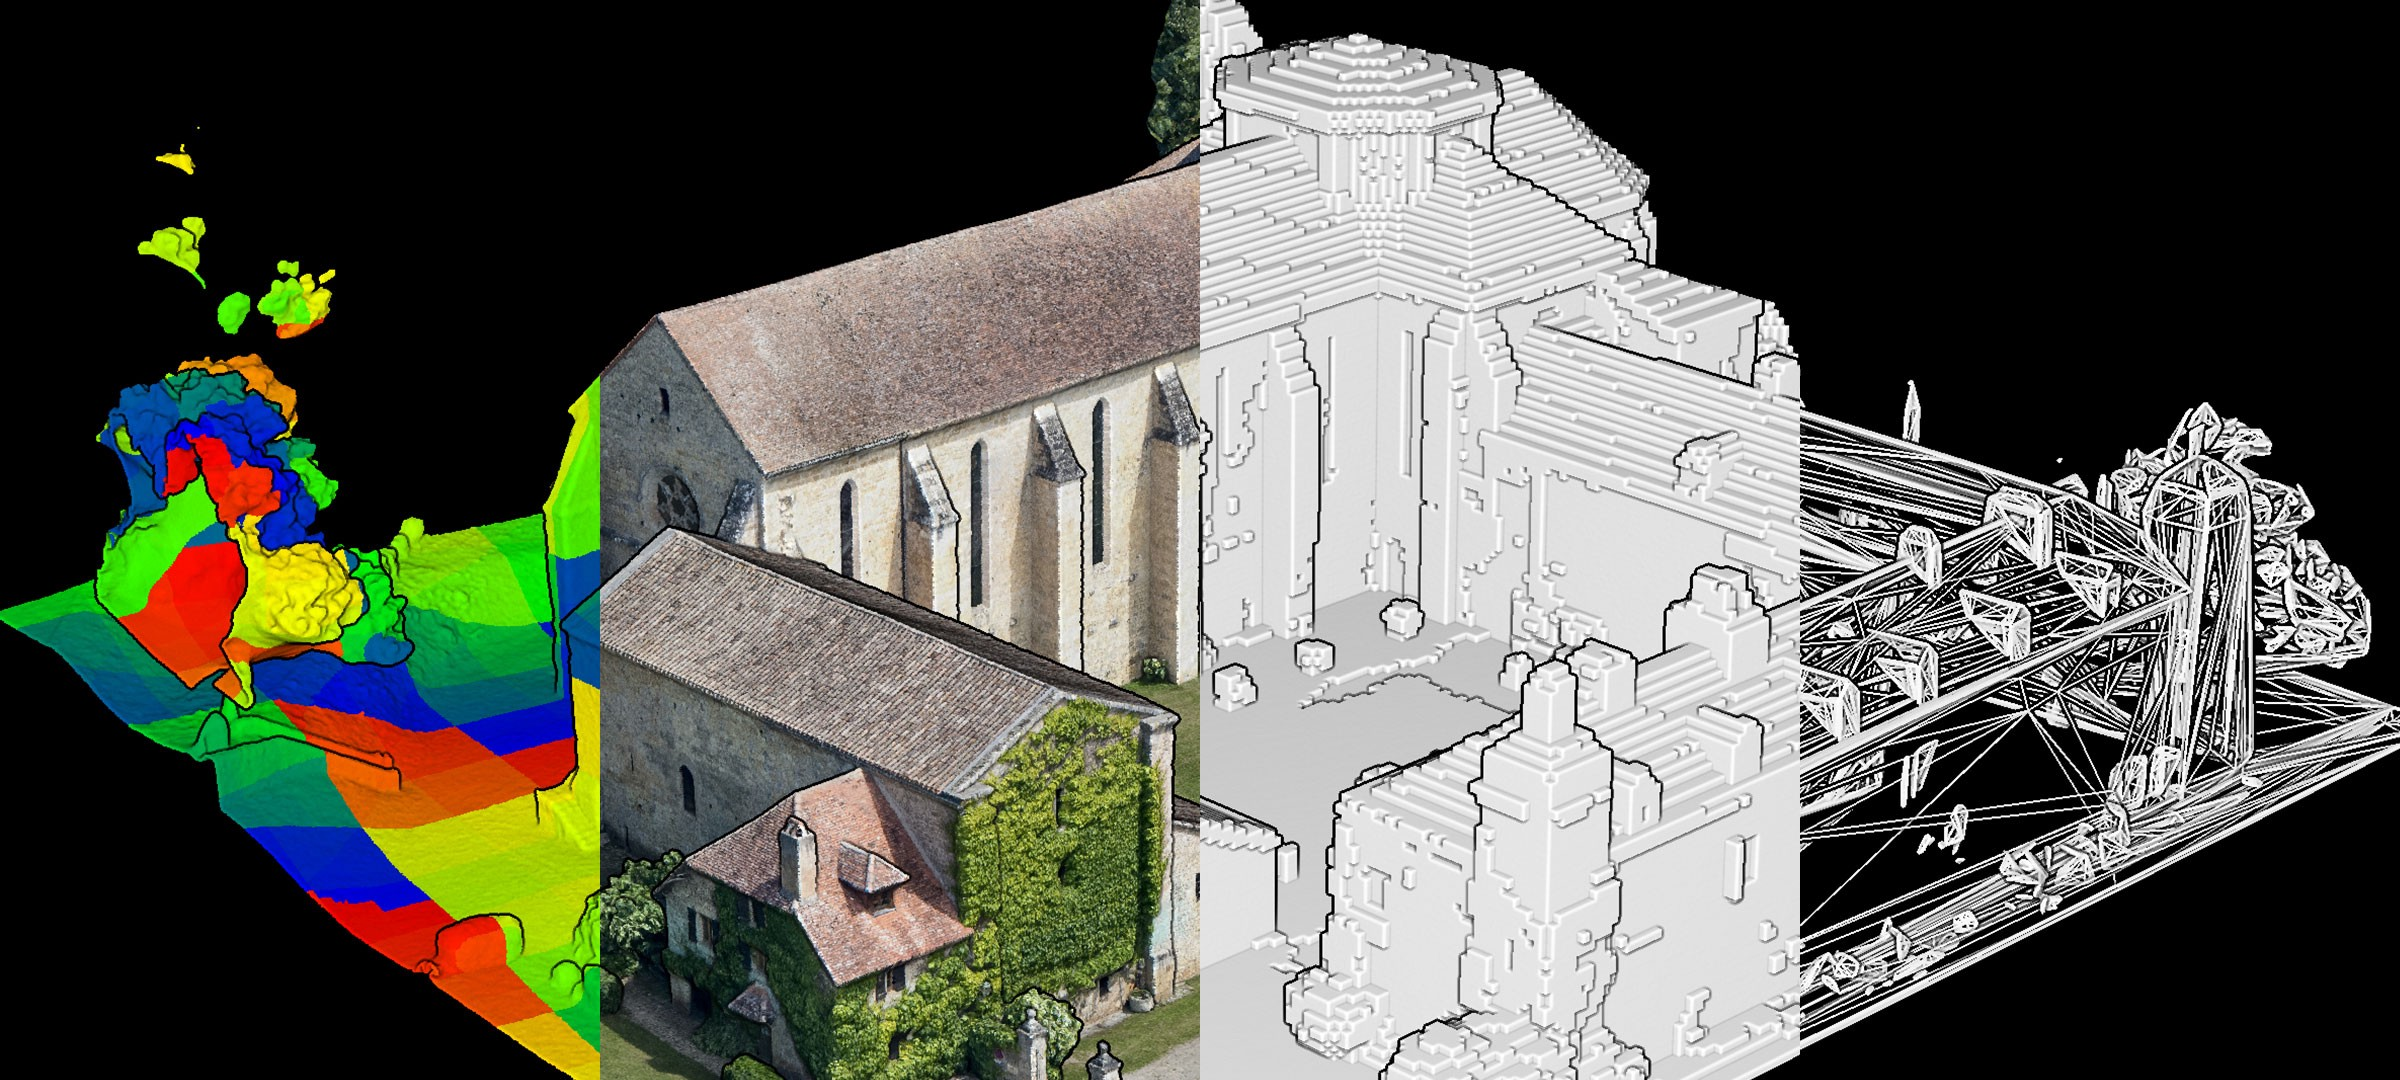
\includegraphics[width=12cm, height=8cm]{3dmodels.jpeg}
        \bigskip
    \\\small\textit{Nota}. Se muestran distintas representaciones de conjuntos de datos 3D. Tomado de \cite{poux-2021} . %citar al frances 
    \end{figure}
    Casi \begin{justifying}
        todos los modelos tridimensionales se pueden dividir en dos categorías: \emph{solidos y caparazón}.
        \begin{itemize}
            \item \emph{Solidos:} definen el volumendel objeto que representa. Muy usados para simulaciones ingenieríles y médicas.
            \item \emph{Caparazón:} representan la superficie/límites del objeto. Usados para crear modelos visuales de captura de movimiento para videojuegos y filmes.
        \end{itemize}
    \end{justifying}
    \vspace{\baselineskip}
    \section{Visualización de objetos}
    Primero \begin{justifying}
        debemos tener la intuición. Acorde a \cite{unknown} %citar eslováca
        la visualización es el tipo de actividad de razonamiento en base al uso de elementos visual o espaciales, ya sea física o mentalmente,
        realizados para resolver problemas o demostrar propiedades.
    \end{justifying}
    Con \begin{justifying}
        ello, debemos tener en cuenta que los elementos para visualizar un objeto tridimensional son parte de la escena tridimensional; específicamente el objeto, las luces y la camara \citep{guan-1999}.\par
    \end{justifying}
    \vspace{\baselineskip}
    \begin{figure}[H]
        \caption{\emph{Elementos básicos de una escena 3D}}
        \centering
        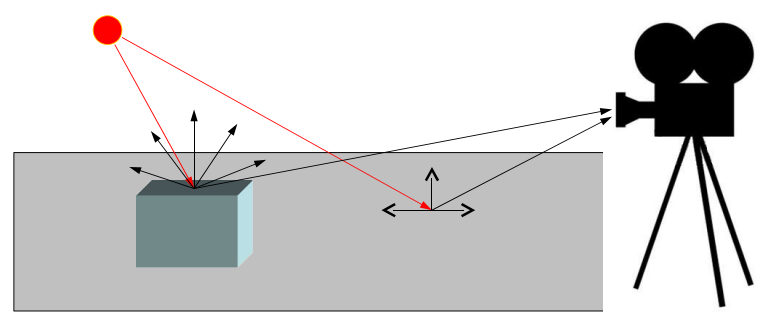
\includegraphics[width=12cm,height=8cm]{3dscene.PNG}
        \bigskip
    \\\small\textit{Nota}. El punto rojo es la fuente de luz y el cubo es el objeto en cuestión. Tomado de \cite{guan-1999}. 
    \end{figure}
    \vspace{\baselineskip}
    \subsection{Objeto}
    En \begin{justifying}
        este, como ya se describió anteriormente, incluye su forma, su localización y su orientación, así como las propiedades de superficie del objeto.\par
    \end{justifying}
    \vspace{\baselineskip}
    \subsection{Luces}
    Se \begin{justifying}
        refiere al punto donde se va a proveer la iluminación. Estos incluyen la posición, ambiente, difusión de la luz en forma de punto fijo, mancha,
        fuente paralela y luz ambiental.\par
    \end{justifying}
    \vspace{\baselineskip}
    \subsection{Cámara}
    También \begin{justifying}
        se le conoce como \emph{espectador}. Sus características incluyen su posición, orientación y su dirección frontal.\par
    \end{justifying}
    \vspace{\baselineskip}
    \section{Transformaciones tridimensionales}
    En \begin{justifying}
        lo competente a tres dimensiones, se clasifican generalmente en 3 tipos: traslación, rotación, escalado \citep{multimedia-applications-division-freescale-semiconductor-inc-2010}.\par %citar el de freescale
    \end{justifying}
    \subsection{Traslación}
    En \begin{justifying}
        esta transformación, todos los puntos o vertices en el objeto se mueven sobre un eje específico \((X, Y \text{ó} Z)\). Su fórmula general es la siguiente:\par
    \end{justifying}
    \begin{equation*}
        \begin{bmatrix}
            x^{\prime}\\
            y^{\prime}\\
            z^{\prime}\\
            1
        \end{bmatrix}=
        \begin{bmatrix}
            1&0&0&t_x\\
            0&1&0&t_y\\
            0&0&1&t^z\\
            0&0&0&1
        \end{bmatrix}
        \begin{bmatrix}
            x\\
            y\\
            z\\
            1
        \end{bmatrix}
    \end{equation*}
    \vspace{\baselineskip}
    \subsection{Rotación}
    Este \begin{justifying}
        se realiza sobre un solo eje. La manera estándar de rotación se realiza usando la convención de mano izquierda.\par
    \end{justifying}
    \subsubsection{Sobre el eje \(X\)}
    \begin{equation*}
        \begin{bmatrix}
            x^{\prime}\\
            y^{\prime}\\
            z^{\prime}\\
            1
        \end{bmatrix}=
        \begin{bmatrix}
            1&0&0&0\\
            0&\cos \theta&-\sin \theta&0\\
            0&\sin \theta&\cos \theta&0\\
            0&0&0&1
        \end{bmatrix}
        \begin{bmatrix}
            x\\
            y\\
            z\\
            1
        \end{bmatrix}
    \end{equation*}
    \vspace{\baselineskip}
    \subsubsection{Sobre el eje \(Y\)}
    \begin{equation*}
        \begin{bmatrix}
            x^{\prime}\\
            y^{\prime}\\
            z^{\prime}\\
            1
        \end{bmatrix}=
        \begin{bmatrix}
            1&0&0&0\\
            0&\cos \theta&-\sin \theta&0\\
            0&\sin \theta&\cos \theta&0\\
            0&0&0&1 
        \end{bmatrix}
        \begin{bmatrix}
            x\\
            y\\
            z\\
            1
        \end{bmatrix}
    \end{equation*}
    \vspace{\baselineskip}
    \subsubsection{Sobre el eje \(Z\)}
    \begin{equation*}
        \begin{bmatrix}
            x^{\prime}\\
            y^{\prime}\\
            z^{\prime}\\
            1
        \end{bmatrix}=
        \begin{bmatrix}
            \cos \theta&-\sin \theta&0&0\\
            \sin \theta&\cos \theta&0&0\\
            0&0&1&0\\
            0&0&0&1
        \end{bmatrix}
        \begin{bmatrix}
            x\\
            y\\
            z\\
            1
        \end{bmatrix}
    \end{equation*}
    \vspace{\baselineskip}
    \subsection{Escalado}
    Especificamente \begin{justifying}
        nos referimos a los escalados uniformes. Su representación matricial es la siguiente:\par
    \end{justifying}
    \begin{equation*}
        S=\begin{bmatrix}
          s_x&0&0&0\\
          0&s_y&0&0\\
          0&0&s_z&0\\
          0&0&0&1  
        \end{bmatrix}
    \end{equation*}
    \vspace{\baselineskip}
    \section{Conclusión}
    Los \begin{justifying}
        temas vistos permiten tener unos fundamentos sólidos para poder aplicar sin problemas la graficación tridimensional
        en lo correspondiente a la materia.\par
    \end{justifying}
    
    \newpage   
    % Referencias
    \renewcommand\refname{\textbf{Referencias}}
    \bibliography{referencias}
    
\end{document}